% -*- coding: utf-8 -*-
\documentclass{article}

\usepackage{listings}
\usepackage{ctex}
\usepackage{graphicx}
\usepackage[a4paper, body={18cm,22cm}]{geometry}
\usepackage{amsmath,amssymb,amstext,wasysym,enumerate,graphicx}
\usepackage{float,abstract,booktabs,indentfirst,amsmath}
\usepackage{array}
\usepackage{booktabs} %调整表格线与上下内容的间隔
\usepackage{multirow}
\usepackage{diagbox}
\usepackage{subfigure} 
\usepackage[colorlinks,linkcolor=blue,urlcolor=black,anchorcolor=blue,citecolor=blue,]{hyperref}%超链接包
\renewcommand\arraystretch{1.4}
\usepackage{indentfirst}
\setlength{\parindent}{2em}

\geometry{left=2.8cm,right=2.2cm,top=2.5cm,bottom=2.5cm}
%\geometry{left=3.18cm,right=3.18cm,top=2.54cm,bottom=2.54cm}

\graphicspath{{figures/}}

\title{\heiti 实验二:绘制比较语料库GENIA和AGAC的词云 }

\begin{document}

	\maketitle
	
	\vspace{5cm}
	
	\begin{table}[h]
		\centering
		\begin{Large}
			\begin{tabular}{p{3cm} p{7cm}<{\centering}}
				学  \qquad  校: &  华中农业大学     \\ \cline{2-2}
				学院班级:      & 信息学院生信1801班   \\ \cline{2-2}
				姓  \qquad  名: & 邓启东 \\ \cline{2-2}
				学  \qquad  号: & 2018317220103 \\ \cline{2-2}
				指导教师:       &夏静波 \\ \cline{2-2}
			\end{tabular}
		\end{Large}		
	\end{table}
	
	\newpage%一个新的页面

	\tableofcontents
	
	\newpage
\section{实验目的}
\subsection{前期工作}
在之前的作业一中我们已经衡量了两个语料库的TTR(类符/形符比),并且分析了两个语料库的TTR衡量可能存在的问题。并且在考虑后引入了STTR(标准化类符/形符比),排除了语料库长度造成的影响,两个语料库得到了近乎一致的结果。
\subsection{本次实验}

本次实验我们会对语料库中出现的词语的词汇频率进行统计,并且采用词云的方式可视化呈现。我们首先简单的使用了已有的R代码绘制得到了一个简单的词云。然后分析其结果存在的词语重复问题,采用python的jieba包进行分词,nltk包进行词干提取,然后用Python的wordcloud包进行更加丰富的词云图片绘制。
\section{实验材料}
\subsection{实验所需包及语料库}
上半部分:\par
R语言的tm\_map文本挖掘包、wordcloud词云绘制包、GENIA语料库、AGAC语料库(均处理成单行词语)。\par
下半部分:\par
python的jieba包进行分词,nltk包进行词干提取,然后用Python的wordcloud包进行更加丰富的词云图片绘制。
\subsection{词云图介绍}
wordcloud,也叫词云图,也叫文字云,是对文本中出现频率较高的“关键词”予以视觉化的展现,词云图过滤掉大量的低频低质的文本信息,使得浏览者只要一眼扫过文本就可领略文本的主旨。
\subsection{语料库介绍}
	\subsubsection{GENIA语料库}
  GENIA语料库是一个生物医学文献集合。这个语料库是为了发展和评估分子生物学信息检索及文本挖掘系统而创建的。GENIA corpus version 3.0.包含2000篇来自MEDLINE数据库的摘要。这些摘要是由PubMed按照human、blood cells以及transcription factors三个医学主题词(medical subject heading terms )为搜索条件搜索到的。这个语料库已经被按照不同级别的语言信息、语义信息进行标注。

其包含:

1. 词性标注2.短语结构句法注释4.事件注释5.关系注释6.指代消解注释(跨句结构里面,代词到底指的是什么)
\href{http://www.nactem.ac.uk/GENIA/current/GENIA-corpus/Part-of-speech/GENIAcorpus3.02p.tgz}{\underline{(GENIA下载链接)}}
	\subsubsection{AGAC语料库}
AGAC(Annotation of Genes with Alteration-Centric function changes)是一个活性基因人类专家注释语料库,目的是捕捉突变基因在致病环境中的功能变化。可以用于药物再利用的案例研究,揭示了变异与广泛的人类疾病之间的潜在关联。AGAC注释了11种命名实体类型。通过识别出LOF/GOF分类的基因-疾病关联,结合LOF-激动剂/ GOF-拮抗剂假说可以应用于疾病候选和物质的知识片段的发现。
\href{http://pubannotation.org/collections/AGAC}{\underline{(AGAC下载链接)}}

\section{实验步骤}
\subsection{语料库处理}
\subsubsection{GENIA语料库过大问题及解决}
在统计过程中,由于本地电脑的内存有限,而GENIA语料库太大,电脑再将变量dtm转换成矩阵的时候无法分配大小为36.7 Gb的矢量。\par
因此我们书写代码(见代码 get\_GENIA.py)将GENIA截取前55,414行,和AGAC的行数保持一致(保存为 get\_part\_of\_GENIA.txt文件)。\par
这种方式其实有一个问题就是不是随机抽取行,可能会因为文献顺序问题影响结果,不能反映GENIA全文的词频。不过随机抽行也很简单,这里知识以截取前55,414行作为示例进行分析。
\subsection{词频统计及绘图}
之前的TTR和STTR的计算都是为了观察语料库的复杂程度,也就是词语不重复的程度。为了直观地观察两个语料库重复的词语的程度,我们使用R语言的tm\_map这个文本挖掘包对语料库中出现的词语进行统计。

之后过小写转换、去掉数字、去除停用词(the/of/a之类的无实义的词语)、去除标点、空格之后进行词语频率的统计。
分别得到词频如表\ref{mmm}所示以及词云(见图 \ref{xxaazzz})。\\
\begin{table}[H]
\centering
\begin{tabular}{|c|c|c|c|}
\hline
\multicolumn{2}{|c|}{GENIA} & \multicolumn{2}{c|}{AGAC} \\ \hline
word              & freq    & word           & freq     \\ \hline
cells             & 673     & mutations      & 373      \\ \hline
kappa             & 453     & function       & 363      \\ \hline
cell              & 442     & mutation       & 260      \\ \hline
expression        & 340     & loss           & 213      \\ \hline
binding           & 305     & gene           & 209      \\ \hline
gene              & 298     & cells          & 187      \\ \hline
alpha             & 298     & expression     & 173      \\ \hline
protein           & 285     & mutant         & 168      \\ \hline
activation        & 258     & protein        & 167      \\ \hline
transcription     & 244     & variants       & 167      \\ \hline
\end{tabular}
\caption{两语料库出现频率较高的前十个词汇极其出现次数}
\label{mmm}
\end{table}

\begin{figure}[H]
  \centering
  \subfigure[GENIA词云]{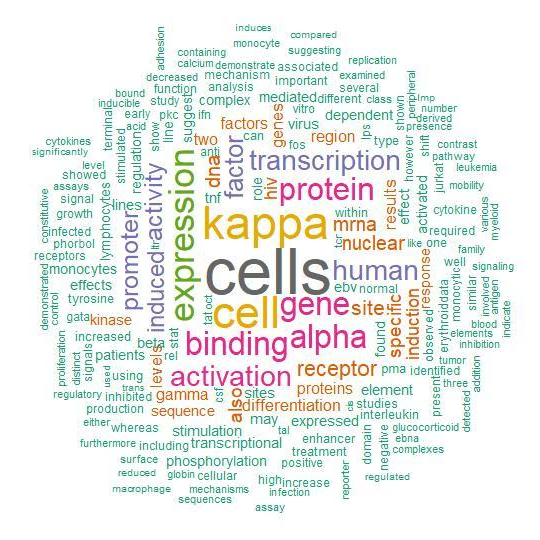
\includegraphics[width=3.1in]{picture/GENIA_wordcloud.png}}
  \subfigure[AGAC词云]{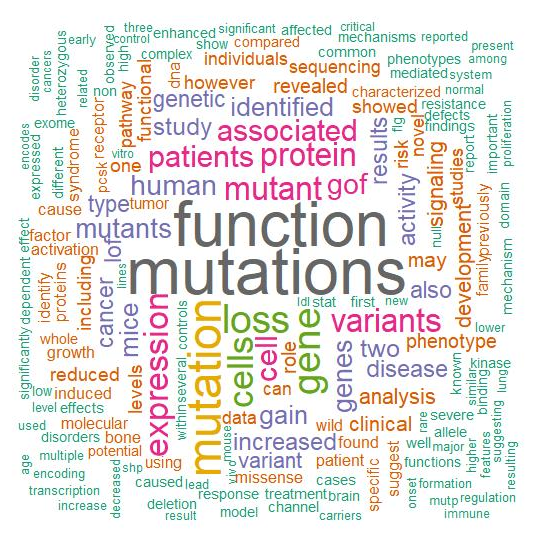
\includegraphics[width=3.1in]{picture/AGAC_wordcloud.png}}
  \caption{R包wordcloud绘制结果}
  \label{xxaazzz}
\end{figure}



\subsection{词云结果分析}
GENIA词云分析:\par
我们可以从高频词表和词云图看出,两个语料库的高频词汇有所区别。很明显,GENIA语料库中出现的高频词有"cell"、"gene"、"transcription"、"protein"、"human"等。\par
前文提到,GENIA语料库本身是在Pubmed上根据的三个医学主题词:human、blood cells以及transcription factors得到的2,000篇摘要。这里的词云高频词和检索使用的主题词呈现出相似性。\par
而出现频率最高的"cells"这个词我们理解为这些文献的生物系统尺度主要是细胞层面的。实际上,cells作为一个常见词,出现的频率最高也是可以理解的。\par
对于其中出现的一个出现频次也很多的词"kappa",经过原始摘要检查发现实际指的是"NF-kappa-B",即一种核因子蛋白,一个转录因子蛋白家族。在几乎所有的动物细胞中都能发现NF-kB,它们参与细胞对外界刺激的响应,如细胞因子、辐射、重金属、病毒等。在细胞的炎症反应、免疫应答等过程中NF-kB起到关键性作用。NF-kB的错误调节会引发自身免疫病、慢性炎症以及很多癌症。NF-kB也与突触的可塑性、记忆有关。\par
AGAC词云分析:\par
AGAC语料库中出现的高频词是"mutations"、"mutations"、"function"、"loss"、"gene"等词语。可以明显看出其是关于突变基因和功能变化的语料库。和我们的预期一致。"loss"、"gof"等词也是后续我们实体识别中需要贴上标签的词汇。
\subsection{存在的问题}
首先,R语言处理GENIA语料库的时候会有内存问题,只能处理语料库的一部分。\par
其次,我们看到绘制出的词云存在无法区分"mutations","mutant"及"mutation"的问题。除此以外的例子还有"cells"和"cell","genes"和"gene"等等。即单复数,词性无法区分,导致两个词语的语义相近或一致却分别计数。要想解决这个问题,则需要nltk包的词干提取器进行词干提取。
\subsection{改进:python nltk包词干提取}
我们将原语料库的文本进行以下处理:1.把标点符号(除"-"')都替换成空格;2.多个空格替换成一个空格;3.单词转换成小写;4.数字替换成"NBR"。得到单个单个的小写词语语料库。分别保存为GENIA.txt和AGAC.txt。这样其实已经按照句子拆分开了,不再需要tokens = tk.word\_tokenize(text)函数进行按句拆分。发现处理后GENIA语料库共有407,120个词。
\subsubsection{三种词干提取器对比}
我们分别使用nltk包的三种词干提取器,并进行每个词语的词干抽提结果打印,其部分结果如下(见图\ref{xxxxxxx}):
\begin{figure}[H]
  \centering
  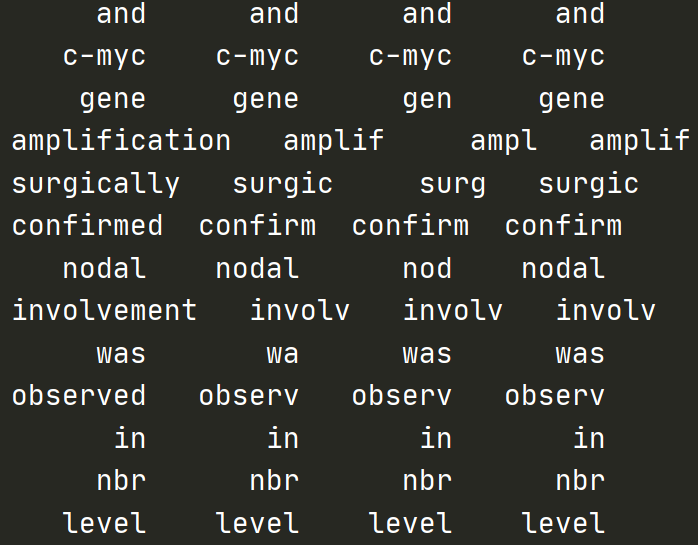
\includegraphics[scale=0.5]{./picture/词干提取.png} %1.png是图片文件的相对路径
  \caption{词干提取结果} %caption是图片的标题
  \label{xxxxxxx} %此处的label相当于一个图片的专属标志,目的是方便上下文的引用
\end{figure}
结果分为四列,从左至右分别是波特词干提取器、兰卡斯词干提取器、思诺博词干提取器。整体感觉兰卡斯词干提取器抽提的词干更加具体,更小一些,甚至把"gene"替换成了"gen"。\par
考虑到我们只是想要区分一些单复数,也想尽可能的保留完整的语义,经过粗略的观察,最终决定使用思诺博词干提取器。\par
其实还可以使用词型还原器将复数名词还原成单数名词,分词还原成动词原型。这里抽取了词干,便不再需要进行词性还原操作了。
\subsubsection{图形绘制}
python版本的worldcloud包功能十分强大,不仅可以自选字体、颜色。更重要的是可以选择背景图片,结果如下图(图\ref{zczxzx})。
\begin{figure}[H]
  \centering
  \subfigure[背景图片1]{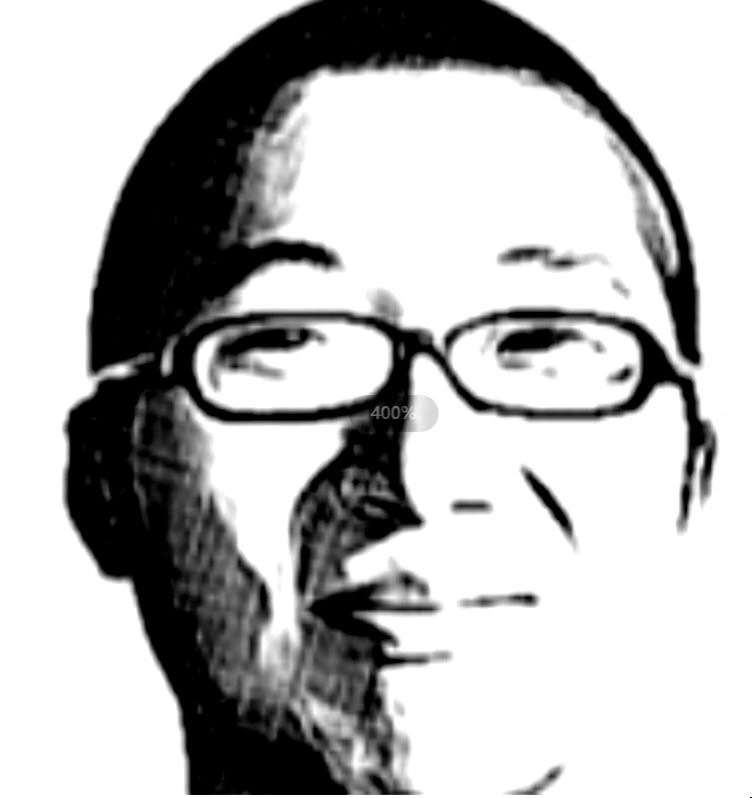
\includegraphics[width=3in]{picture/源头像.JPG}}
  \subfigure[GENIA词云]{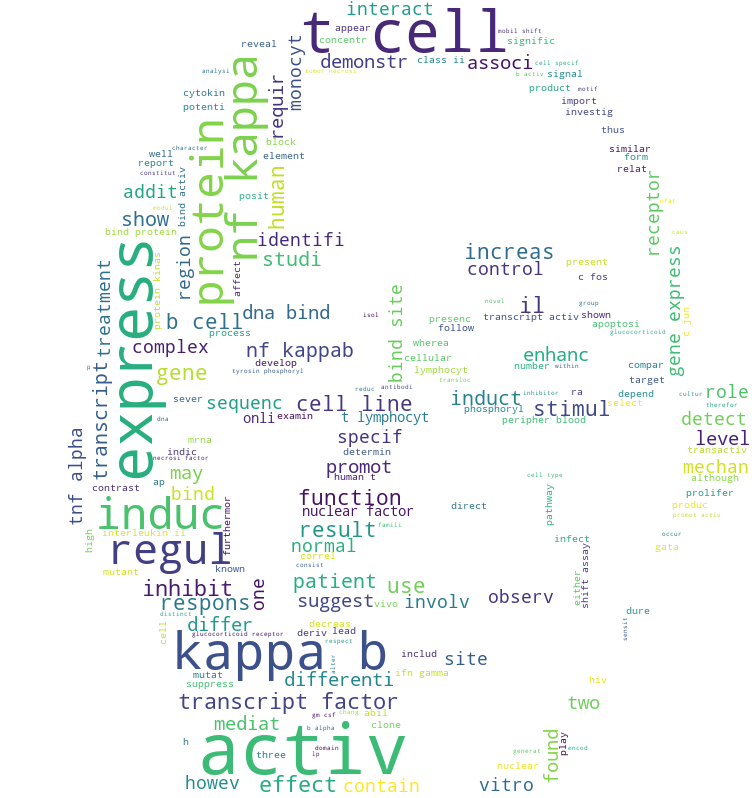
\includegraphics[width=3in]{picture/result.png}}
  \caption{GENIA词干wordcloud结果}
  \label{zczxzx}
\end{figure}
为了生动充分地展示其效果,我们在未经老师本人授权的情况下,盗用了老师的面部照,光明正大地侵犯了老师的肖像权(<( ̄︶ ̄)>)。\par
这个时候我们发现和之前简单的R包处理结果相比较,高频的词干都比较眼熟,比如"regul"应该指的是"regulation",而"active"$\rightarrow$"activation"、"express"$\rightarrow$"expression"、"induc"$\rightarrow$"induction"、"kappa"依然保留,"cell"不再有复数形式同时存在。不过由于变成了词干,词语的相对出现频次有所改变,因此相对大小不再像以前一样。
\begin{figure}[H]
  \centering
  \subfigure[背景图片2]{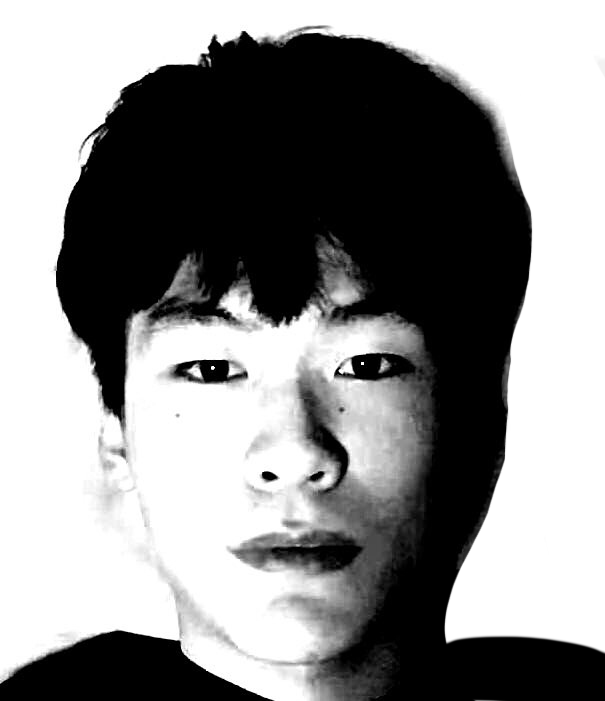
\includegraphics[width=3in]{picture/Deng.png}}
  \subfigure[AGAC词云]{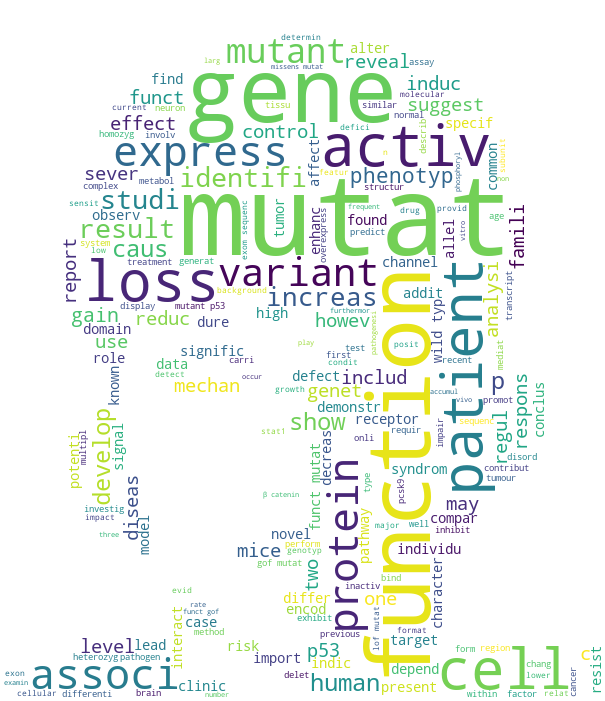
\includegraphics[width=3in]{picture/Dengresult.png}}
  \caption{AGAC词干wordcloud结果}
  \label{sssdddd}
\end{figure}
AGAC也是如此,该有的"associ"$\rightarrow$"association"、"mutat"$\rightarrow$"mutation"、"functions"$\rightarrow$"function"、"activ"$\rightarrow$"activate",这里不再详细赘述。
\section{实验总结}
词云绘制给了我们一个方便而直观的方式看到语料库的高频词,通过词云图片让我们对其主题有一个大概的把握。\par
原本本次实验仅仅停留在3.3,R代码跑通就结束了。但是本着精益求精以及娱乐的方式,整个项目从头用python实现并且进行了进一步的词干提取和背景选取。整个呈现便丰富了很多。这其实就是学习的一个过程。\par


\end{document}













